Results:
	-Total active days pre+post-trimming
	-Total count of sp events (also pre+post?)
-Overall detection rate pattern in all species
-Overall activity pattern in all species
-Density curves throughout the year, obs per (week/month)
-Intro to how each sp will be presented

Sp:
-Nth most common with n events,
	-at n of the 56 sites 
- activity pattern
	-compared to expected activity from literature (cite)
	-LED exposure (ie. activity during night
	(-activity-density with and without event-filter?)
-The model
	-TK parameter(s) was (non-|significant) in SNHT (see table \ref{tab:param})
	-Equivalence test says (mention 2nd gen p-value)
	-ggeffects plot shows...
-Conclusive sentence on species





The type of CT flash had an overall minor effect on detection rates.
In general, the control periods (which never had white flashes) had a somewhat lower detection rate than the IR and wLED periods.
%Between the experiment periods, I expected the IR periods to have the highest detection rate, but LED was somewhat higher for most species (see table \ref{tab:params}). %AMkomm: why?

There were a total of TK camera trapping days, which was unevenly distributed between the different periods and period types. Trimming the data according to median period length of IR periods (which was shorter than that of control and wLED periods) evened out the disproportions between the periods (see figure \ref{fig:active days}).

\begin{figure}
 \centering
	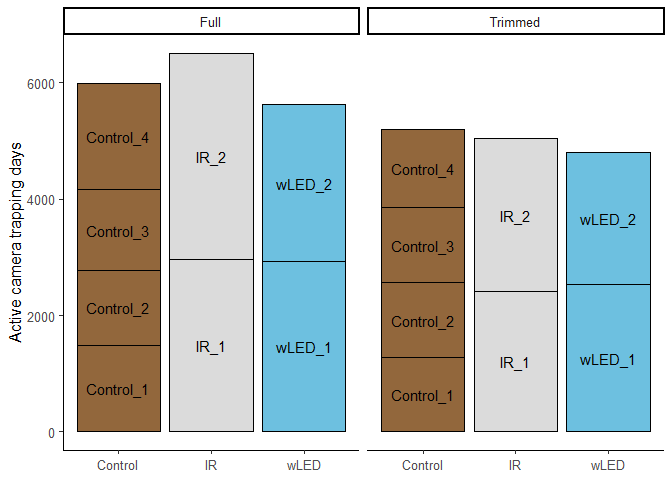
\includegraphics[scale=.9]{../R/glmm_sp_files/figure-html/active-days-3.png}
 \caption[Active camera days]
 {Active camera days %\par \small
 Number of active days per type of period, before and after trimming the data}
 \label{fig:active days}
\end{figure}


%
%\begin{figure}
% \centering
%	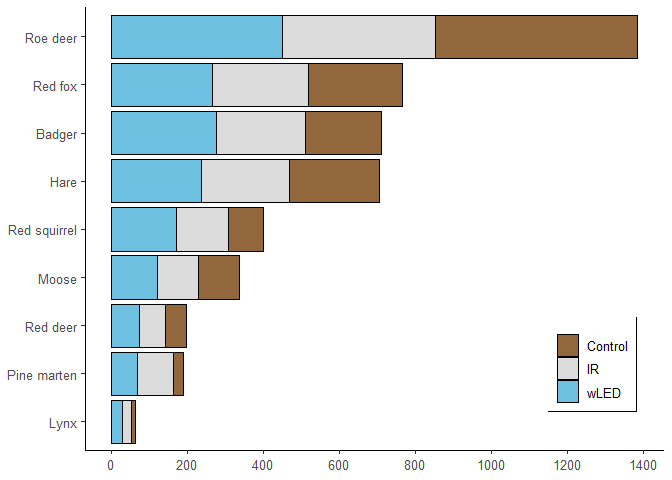
\includegraphics[scale=.9]{../R/glmm_sp_files/figure-html/events-1.png}
% \caption[Total number of events per species]
% {Total number of events per species}
% \label{fig:events}
%\end{figure}


\begin{figure}
 \centering
	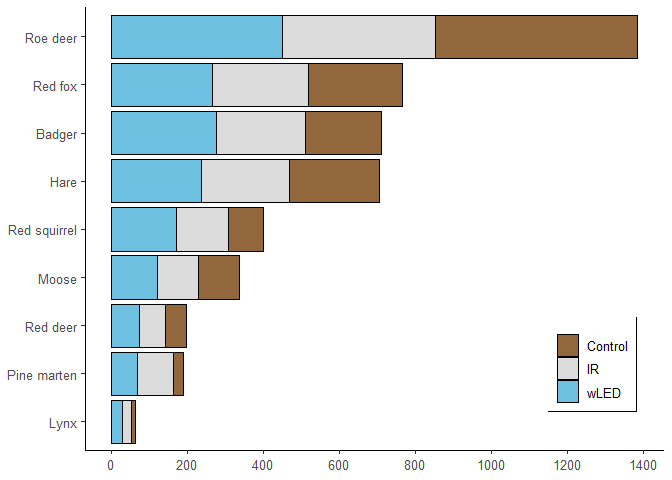
\includegraphics[scale=.9]{../R/glmm_sp_files/figure-html/events-1.png}
 \caption[Raw count and number of events per species]
 {Raw count and number of events per species}
\end{figure}





\subsection{SP}

SP was nth most common with n events.
SP was active during 
ie. most photos were taken during (night-time/daylight), as visualised in figure \ref{fig:SP}c.
The overall pattern was TK between each group (Control, IR, LED), which means that the overall effect of white LED ...
The GLMM explaining variation in detection rate of SP had a substantial explanatory power (conditional R2 = 0.xx), but the part related to the fixed effects alone (marginal R2) is just 0.00x.
In other words, most of the explained variation in detection rate was due to seasonal changes and variation between the different camera sites captured in the random terms.

In a standard null hypothesis significance test (NHST) the effect of white LED was TK significant, and TK parameters were considered significant.

Looking at figure \ref{fig:SP}a, the detection rate of SP was generally lower(?) in the control group than for the two treatment groups, and TK had the highest rate.
The slope for control group is approximately horizontal (?), and the slopes of the treatment groups...

Considering the equivalence test, which also is a visualisation of the numbers in \ref{tab:params}, the large variation in IR/LED...

The interaction with time since deployment is(n't) practically equivalent with the slope of Control.






